% KJGNOTE: PLEASE SEE BOTTOM OF DOCUMENT FOR BLOCK COMMENTS
\documentclass[a4paper,12pt]{article} % must always appear at start of every document
% alternative classes to "article": report, proc, book, slides

\usepackage{color} % allows color to be used
\usepackage[margin=2cm]{geometry} % attempt to control margin width on pages (can be "in" or "cm")
\usepackage[utf8]{inputenc} % allows german characters
\usepackage{mathptmx} % this package makes the font look closest to Times New Roman
\usepackage{csvsimple} % lets you import a csv file to make, say, a table
\usepackage{graphicx} % required to load images into image

\usepackage{chngcntr} % enables per-section numbering of any captions
\counterwithin{figure}{section} % per-section numbering, figures
\counterwithin{table}{section} % per-section numbering, tables
\counterwithin{equation}{section} % per-section numbering, equations
\usepackage{hyperref} % allows you to hyperlink to other sections in a document

% anything before \begin{document} is considered "Preamble"

% DOC START ====================================================================
\begin{document}
\title{Summary of LaTeX Features \\
(following ``LaTeX for Beginners'')}
\author{Kris Gonzalez, John Deere} 
\date{2018-10-25}
\date{October 25,2018}
\date{15.01.2019} % can also be "October 25, 2017" or "2018-10-25" if desired, only treated as string
\maketitle % necessary to have title page on first page
\pagenumbering{gobble} % turns off page numbering when you don't want it

%  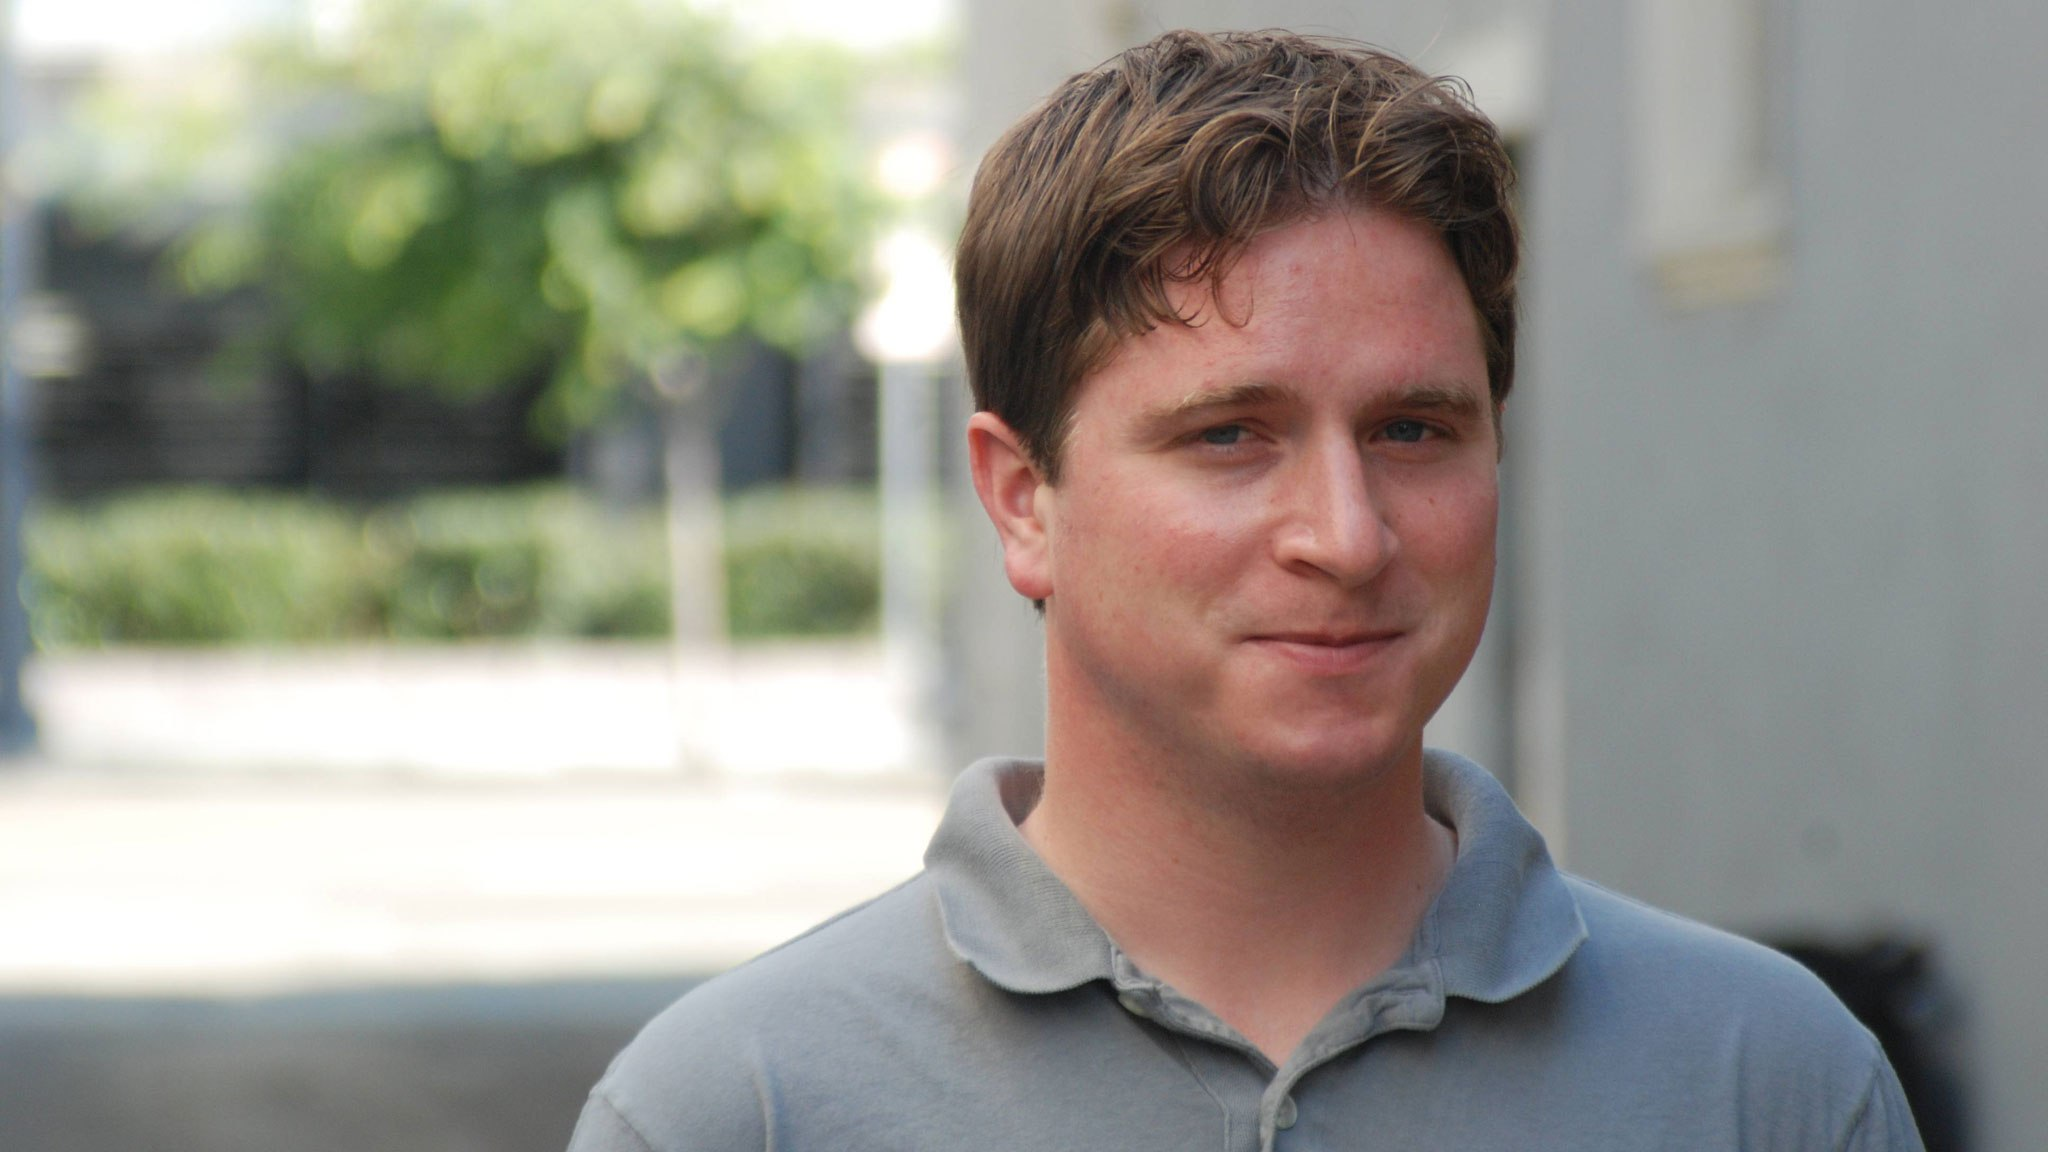
\includegraphics[width=1\textwidth]{media/titleimg.jpg} 
% note, you need width=0.5 if dealing w/ two columns

\newpage
% TABLE OF CONTENTS ============================================================
\pagenumbering{roman}
\tableofcontents

%\twocolumn % enables two or \onecolumn (default) behavior

% SECTION ======================================================================
\newpage
\pagenumbering{arabic} % can use initial things to 
\section{Introduction}
\label{Introduction}
So, this document accompanies the pdf ``Latex for Beginners'' which can be found at the following link: www.google.com. This document will generally follow  the same order as the pdf. Any special commands will be included at the end. General structure of the supplemental PDF: 
\begin{itemize}
\itemsep=-0.5em
\item Creating a Title
\item Sections
\item Labelling
\item Table of Contents
\item Typsetting Text
\item Lists
\item Comments \& Spacing
\item Special Characters
\item Tables
\item Figures
\item Equations
\item References
\item Special Commands (kjg own section)
\end{itemize} % list

So, let's get started. 

% SECTION ======================================================================
\section{Document Structure} \label{Document Structure}
\subsection{Basic document} \label {Basic document}
Each document requires a few things, given as examples below (in order of appearance): 

\begin{itemize}
\itemsep=-0.5em
\item \textbackslash documentclass[a4paper,12pt]\{article\} : defines what the document's like (*)
\item \textbackslash usepackage\{chngcntr\}                 : imports helpful packages
\item \textbackslash counterwithin\{equation\}\{section\}   : enables numbering on figures, etc
\item \textbackslash begin\{document\}                      : end of preamble, start of main body (*)
\item \textbackslash section\{SectionName\}                 : section title
\item \textbackslash label\{SectionLabel\}                  : linkable / reference for each (sub)section
\item \textbackslash subsection\{SubsectionName\}           : subsection title
\item \textbackslash end\{document\}                        : end of body, start of post-body (*)
\end{itemize}

Each of these are important for the document to function properly, but only three are essential [marked with (*) ]. The document can be roughly divided into 3 parts: preamble, body, and post-body (kjg name). the preamble is for package loading and initializations; the body is for actual content, and the post-body is for comments / non-printed stuff (anything can be written here, not put in final document).

\subsection{Title Page / Initial Commands}
Main commands that are needed: 

\begin{itemize}
\itemsep=-0.5em
\item \textbackslash title
\item \textbackslash author
\item \textbackslash date
\item \textbackslash maketitle
\item \textbackslash pagenumbering
\item \textbackslash maketitle
\item \textbackslash pagenumbering\{gobble\}

\end{itemize}



\newpage
\onecolumn

% SECTION: Basic Formatting ====================================================
\section{Basic Formatting} \label{Basic Formatting}
So here I am with my own text. Please see section \ref{Basic Formatting} on page \pageref{Basic Formatting} to blah blah blah. Yo, this color text is {\color{red}fire}. lol. Here's a list of font effects:
\begin{itemize}
\itemsep=-0.5em % this is the correct way to reduce the spaces in a list... :)
\item textit = \textit{italics (*sl for \textsl{slanted})}
\item textbf = \textbf{bold}
\item textsc = \textsc{smallcaps}
\item texttt = \texttt{teletype}
\item \{color\{\textit{red}\} ...\} = {\color{red} color}
\end{itemize}

% SUBSECTION: LISTS ============================================================
\subsection{Lists \& Special Characters}
Alright, here we're gonna get serious about lists. here we go. numbered lists:
\begin{enumerate}
\itemsep=-0.5em % this is the correct way to reduce the spaces in a list... :)
\item one
\item two
\begin{enumerate}
\item sublist a (note: this is a pain and the separation is still there
\item sublist b
\end{enumerate}
\item three
\end{enumerate}
Etiam id interdum sem. Proin tempor diam urna, non ultricies est rhoncus ac. Etiam id interdum sem.

Next, bulletlists:
\begin{itemize}
\itemsep=-0.5em
\item one
\item two
\end{itemize}

Note that there are also special characters that have certain meanings in text. quick check for German: ä  ö ü ß . seems like a special package is required, but nothing too bad.

however, there WILL be issues when trying to use a certain set of special characters: 
\\ \\ %two linebreaks
Item \#1A\textbackslash642 costs \$8 \& is sold at a \~{}10\% profit.
\\ \\ %two linebreaks
Etiam id interdum sem. Proin tempor diam urna, non ultricies est rhoncus ac.

% SUBSECTION: TABLES / FIGURES / EQUATIONS =====================================
\subsection{Tables, Figures \& Equations}
Alright, in this section, really want to focus on making good looking figures in our data.

\subsubsection{Tables}
Tables by default are drawn without horizontal and vertical lines...

\begin{table}[h]
\centering
\caption{Mathematical Symbols}
\label{Mathematical Symbols}
\begin{tabular}{|c|c|c|}
\hline
Name & Value & Symbol \\
\hline
pi		& 3.14	& $\pi$ 	\\
e 		& 2.72	& three 	\\
phi		& 1.62	& $\phi$ 	\\

\hline
\end{tabular}
\end{table}

Next, we're gonna spend some time figuring out how to create a table but with numerical data. So, the below is necessary plus some preable lines. Note how you need to place horizontal lines both in the "main" area as well at either top and bottom end. NOTE: tables may be placed on next page, depending on amount of space available.
\begin{table}[h]
\centering
\caption{Random data}
\begin{tabular}{|c|c|}%
\hline
\bfseries Time (s) & \bfseries Zeroed time (s)% specify table head
\csvreader[head to column names]{media/Basket_ball.csv}{}% use head of csv as column names
{\\\hline\csvcoli&\csvcolii}% specify your columns here
\\\hline
\end{tabular}
\end{table}

\newpage
\subsubsection{Figures}
This section to cover how to make figures, which require images to be loaded outside of the file.

\begin{figure}[h] % ahh, h = "approx here", t = "top of page", b = "bottom of pg"
\centering
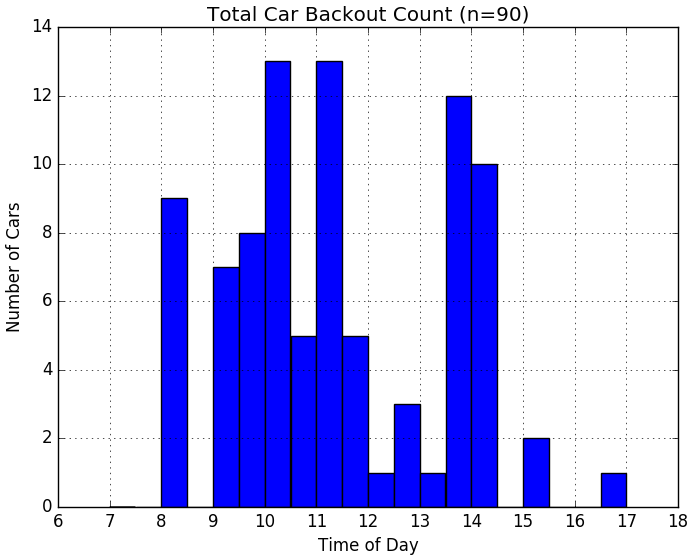
\includegraphics[width=0.5\textwidth]{media/img2.png} % note, you need width=0.5 if dealing w/ two columns
\caption{Loading an image from a subfolder}
\label{figure-parking}
\end{figure}

Not bad, alright so this seems to work nicely. Note the two extra lines that are needed in the preamble to ensure that per-section numbering is used. BUT WAIT, THERE'S MORE: do you want beautiful, zoomable, non pixelated images? then save your graphs to pdf, then import them like so:
\begin{figure}[h]
\centering
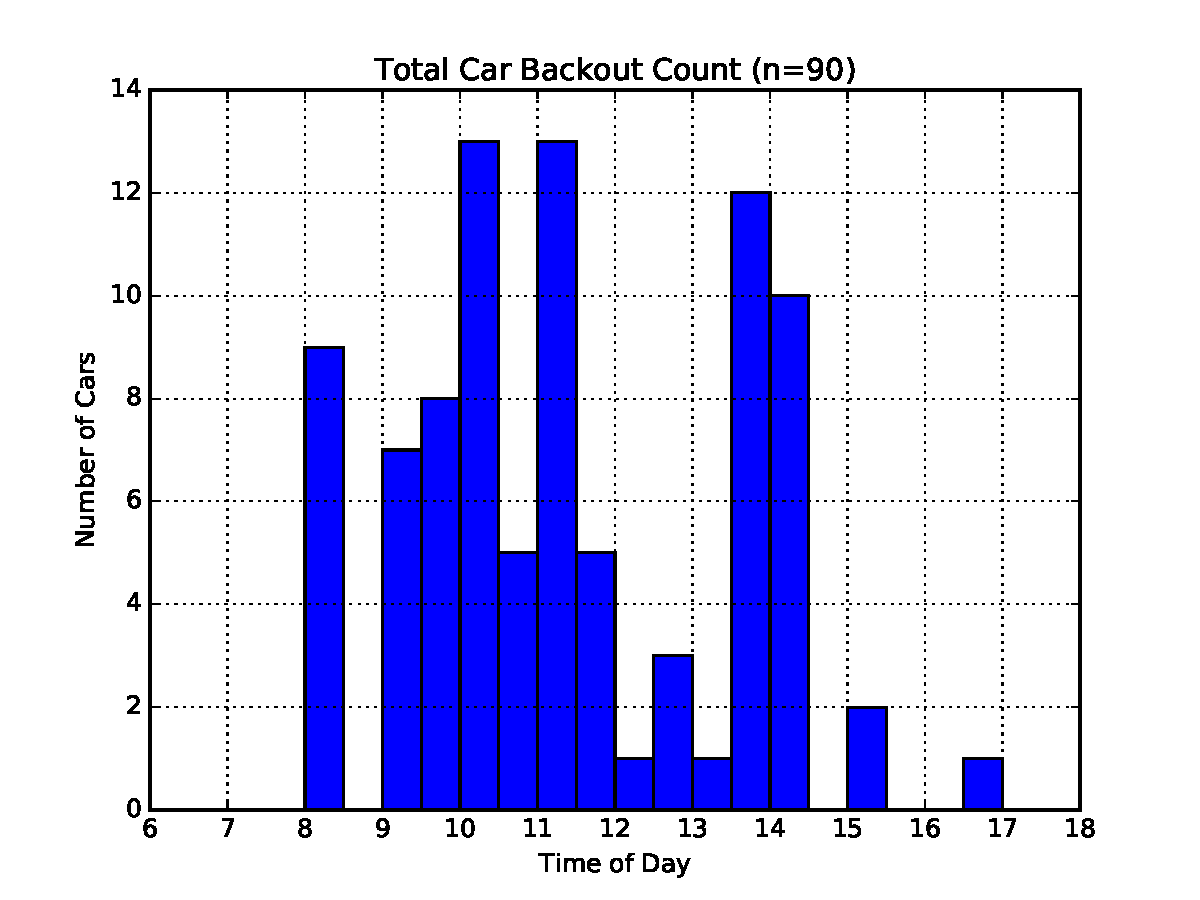
\includegraphics[width=0.5\textwidth]{media/result.pdf}
\caption{Just look at that \textit{NICE} quality.}	
\end{figure}


\subsubsection{Equations}
Alright, now for one of the last special items that interrupt body text: equations. "Math mode" is entered / exited when using a dollar sign, "\$". For example, this equation is in-line: $ f(x)=x^2 $. This next equation has it's own line: $$f(x) = x^3$$ Finally, if we want to add a caption number, we do like so (newline not required):
\begin{equation}
A(r) = \pi/4*d^2
\end{equation}
Note that in order to achieve a (section.equation) format, we need to add more to the preamble. if we want to have multiple equations:
\begin{eqnarray}
a & = & b + c \\ % note that if you wanna align all equal signs, need "&". and every non-last line needs \\
& = & y - z\\
\frac{d(x)}{dt} &=& \ddot x * t \\
v_{esc} &=& \sqrt{\frac{2GM}{R}} \\
\overline x &=& \frac{1}{n}\sum_{i=1}^{n} x_i \\ % note: for product, use \prod
\frac{\sin(x)}{\cos(x)} &=& \tan(x) 
\end{eqnarray} % on last line, leave no spaces and have no newlines

% SECTION ======================================================================
\section{Importing *.tex files for longer documents} \label{sect_teximporting}
This section to be covered by an imported document.
This is the start of the remote section. note that the text begins immediately where the \textbackslash input command is given. We can treat this section just like any other. The other method to use is \textbackslash include, but the big difference here is that it adds a page break. that's not really necessary until you're writing book-length items. with \textbackslash input, you can pretty much treat it as if it were part of the main document, such as with references:

\begin{itemize}
\item Table \ref{Mathematical Symbols} exists behind this document
\item Subsection \ref{super duper} exists ahead of this document
\item three
\end{itemize}

Alright, end of remote section.This text is now part of the main document again. notice how close ``This'' is to the input command

% SECTION: References and Such =================================================
\section{References and Such} \label {sect_references}
So, at this point have about 70\% of the report able to be written. In order to create a set of references (and to cite them), we need a BibTeX file. We eventually want to make a citation, such as to J. Redmon's paper \cite{red16}. Note, however, that getting a bibliography to work is a MASSIVE pain in the ass:
\begin{enumerate}
\itemsep=-0.5em % this is the correct way to reduce the spaces in a list... :)
\item have your document more or less written out
\item insert your references info wherever you \\want it, usually at end (see below in .tex file)
\item refer to your *.bib file in bibliography \\WITHOUT the file extension
\item do some weird mumbo jumbo where you first typeset as  pdfLaTeX, then BibTeX, then back to pdfLaTeX (and rerun typeset as\\  pdfLaTeX a few times)
\item then... it should work... ?
\item OH DON'T FORGET THE LUCK!
\end{enumerate}

MAN WTF NOW THIS LIST WAS OVERRUNNING ITS MARGINS INTO THE OTHER COLUMN????

In any case, let's cover some of the way to cite what we want. the first thing we're gonna cite is this weird ass article, called ahu. ahu to you, \cite{ahu61}. Love ya. anyway, now we move on  to \cite{ab94}, who probably said some really interesting things, but i haven't read it. in any case, notice that articles aren't included unless you actually reference them. and always repeat the above steps when reloading your references: while in your *.tex file: typset as pdflatex, typset as bibtex, then typeset multiple times as pdflatex. 

Next, we're gonna cite two articles that seem to just be different pages of the same thing: \cite{m85} and \cite{m99}. Now, if we wanted to refer to them together, we would refer to them in the same cite tag... no? we'd say we're talking about \cite{m85,m99}.

oh, another thing to note: the references are not in the same order as the bib file. this means that at compilation time, everything is put into some sort of... alphabetical order? not sure.

\subsection{Intra-Document Hyperlinks}
So, we want to refer to other places in the document, but what good are these references if we can't even make them hyperlinks? Let's see here: I want to go to one of the first sections, so please see Section \ref{super duper}. 

UPDATE: wow, ok all you need to do is just import the package "hyperref", and you're done...

Now, another thing we'd probably like to do is arbitrarily link to other things, so why not also use the hypertarget tag: 
i want to return to this \hypertarget{special_word}{word}, and i can refer to it later using the \texttt{hyperlink} tag to go to \hyperlink{special_word}{it}. 
Last test, can i go back to a table by refering to its caption? See Table \ref{Mathematical Symbols}.Yep, it works. Also, let's try referencing a figure, like \ref{figure-parking}


\subsection{Hyperlinks to outside sources}
If you wanna link to somewhere outside the document, especially if you're just *listing* the link, it's a good idea to use \textbackslash href or \textbackslash url, like so: 

\begin{enumerate} \itemsep=-0.5em
\item use "\textbackslash usepackage \{ hyperref \}"
\item include a link with \textbackslash href\{LinkHere\}\{Name\} or just \textbackslash url\{LinkHere\}
\item example: \url{https://www.latex-tutorial.com/tutorials/hyperlinks/} .
\item example2: \href{https://www.latex-tutorial.com/tutorials/hyperlinks/}{Special Name} .

\end{enumerate}


Lorem ipsum dolo. Today's date: \today.
\subsection{super duper}
\label{super duper}
Mauris iaculis id magna 
\subsection{another1}
Mauris iaculis id magna 
\subsection{another2}
Mauris iaculis id magna
\subsubsection{another another}
Mauris iaculis id magna
\paragraph{another still}
Mauris iaculis id magna. 


% BIBLIOGRAPHY =================================================================
\bibliographystyle{plain}
\bibliography{references}
%\references{refs.bib}


% END OF DOCUMENT ==============================================================
\end{document}
% anything typed here is ignored
This section can be used as commenting?

some objectives of learning to use latex: 
* title %done
* table of contents %done
* figures / tables %done
* equations %done
* bullets / numbered lists % done
* changing fonts (monospace) %done
* in-text math % done
* special symbols (math or stuff like ü) % done
* sections %done
* section numbering %done
* paragraph formatting (hanging/firstline/justified/right/etc) % will not pursue
* authors
* bold / italics / underline / etc
* referencing
* citing / cross referencing
* appendices 

= notes / questions while learning:  =======================
* what about multiple authors in the title?
* can't seem to continue page numbering in the middle of a document when have been turned off
* in order to deal with subsections beyond a depth of 3 (e.g. x.x.x.x), check out modifying paragraph: https://tex.stackexchange.com/questions/60209/how-to-add-an-extra-level-of-sections-with-headings-below-subsubsection
* why isn't the first paragraph of each section being automatically indented? 
* to control spacing in a list: %\itemsep=-0.5em % this is the correct way to reduce the spaces in a list... :)
* continuous / persection caption numbering: https://tex.stackexchange.com/questions/28333/continuous-v-per-chapter-section-numbering-of-figures-tables-and-other-docume
* maybe be possible to embed python code directly in a latex document: http://www.texample.net/weblog/2008/oct/24/embedding-python-latex/









% eof